\documentclass[12pt, a4paper]{article}
    
\usepackage{homework}
\usepackage{amsmath}				% For Math
\usepackage{fancyhdr}				% For fancy header/footer
\usepackage{graphicx}				% For including figure/image
\usepackage{cancel}					% To use the slash to cancel out stuff in work
\usepackage{multirow}

%%%%%%%%%%%%%%%%%%%%%%
% Set up fancy header/footer
\pagestyle{fancy}
\setlength{\headheight}{42pt}
\fancyhead[LO,L]{Name: Yu Ching Hei\\SID: 1155193237\\email: chyu2@cse.cuhk.edu.hk}
\fancyhead[CO,C]{}
\fancyhead[RO,R]{CENG3420 Computer Organization and Design\\Lab 3\\Date: \today}
\fancyfoot[LO,L]{}
\fancyfoot[CO,C]{}
\fancyfoot[RO,R]{Page \thepage}
\renewcommand{\headrulewidth}{0.4pt}
\renewcommand{\footrulewidth}{0.4pt}
%%%%%%%%%%%%%%%%%%%%%%

\begin{document}
\begin{qNoMark}
Lab 3.1 result
\end{qNoMark}

\begin{ans}
    \begin{figure}[H]
        \caption{add4 before}
        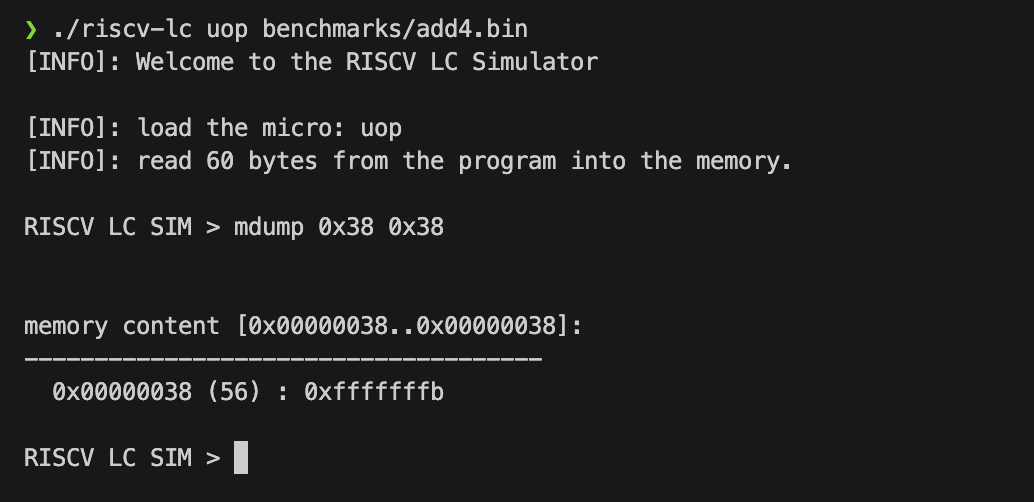
\includegraphics[width=1\linewidth]{../figs/add4-before-1.png}
    \end{figure}
    \begin{figure}[H]
        \caption{add4 after}
        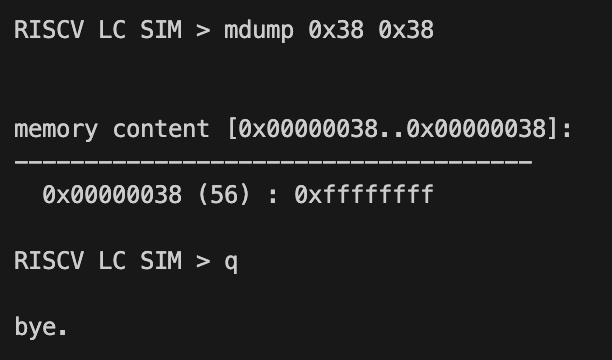
\includegraphics[width=1\linewidth]{../figs/add4-after-1.png}
    \end{figure}
    
    \begin{figure}[H]
        \caption{count10 result}
        \centering
        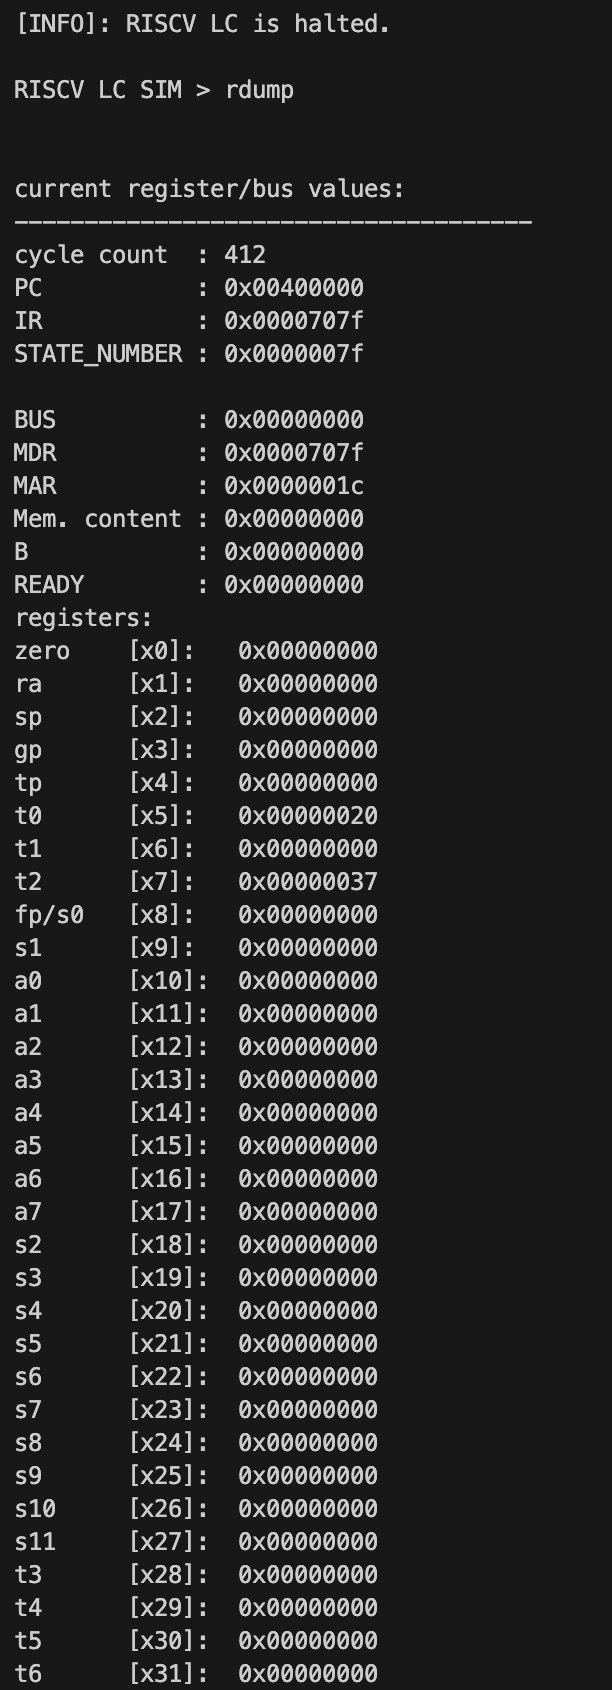
\includegraphics[scale=0.8]{../figs/count10-1.png}
    \end{figure}
    
    \begin{figure}[H]
        \caption{isa register values}
        \centering
        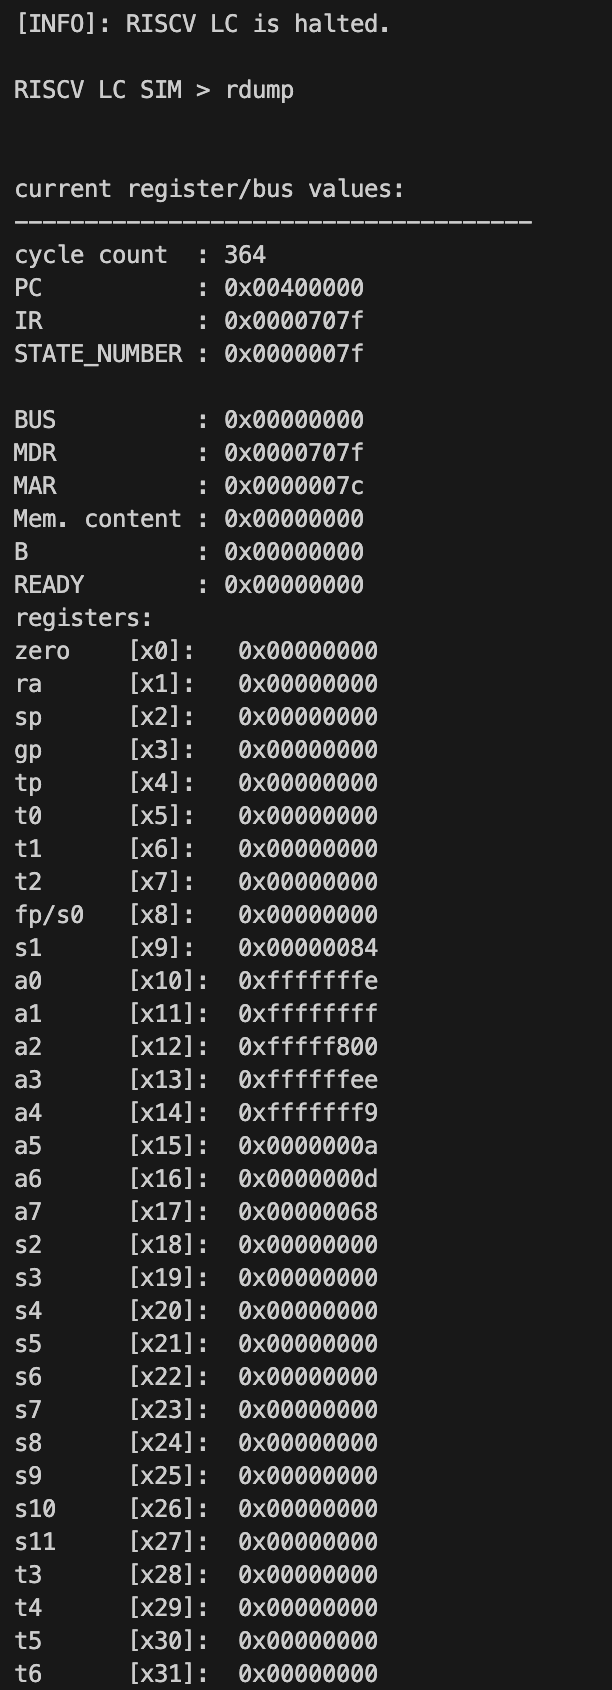
\includegraphics[scale=0.5]{../figs/isa-rdump.png}
    \end{figure}
    \begin{figure}[H]
        \caption{isa memory content}
        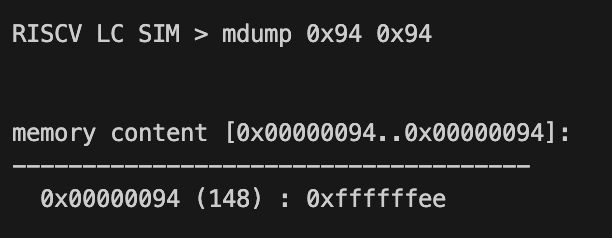
\includegraphics[width=1\linewidth]{../figs/isa-mdump.png}
    \end{figure}
    
    \begin{figure}[H]
        \caption{swap before}
        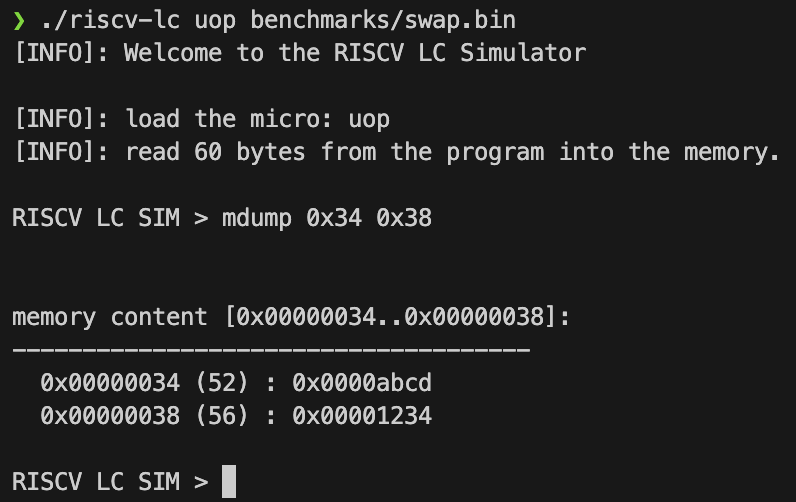
\includegraphics[width=1\linewidth]{../figs/swap-before-1.png}
    \end{figure}
    \begin{figure}[H]
        \caption{swap after}
        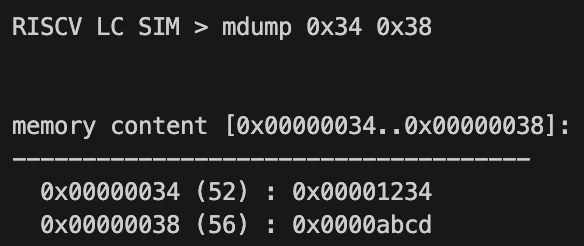
\includegraphics[width=1\linewidth]{../figs/swap-after-1.png}
    \end{figure}
\end{ans}
\pagebreak

\begin{qNoMark}
Lab 3.2 result
\end{qNoMark}

\begin{ans}
    \begin{figure}[H]
        \caption{add4 before}
        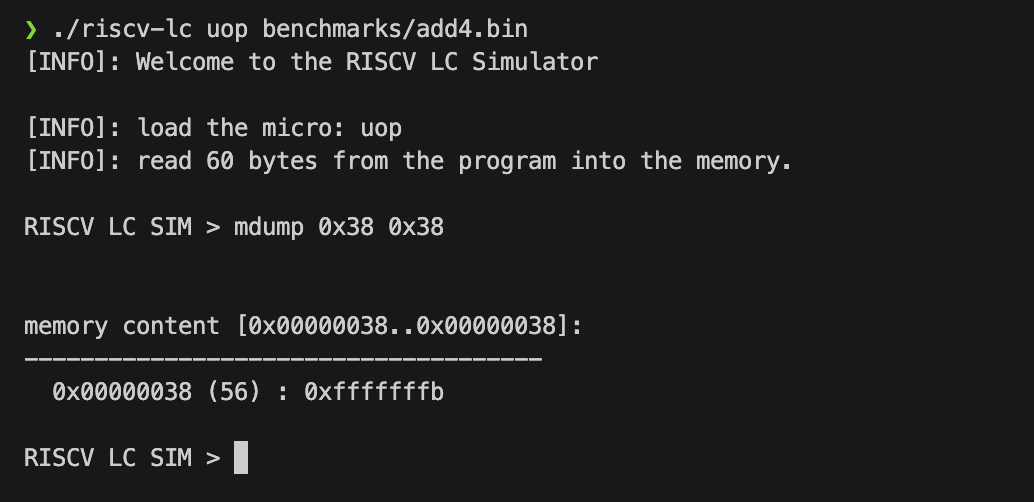
\includegraphics[width=1\linewidth]{../figs/add4-before-1.png}
    \end{figure}
    \begin{figure}[H]
        \caption{add4 after}
        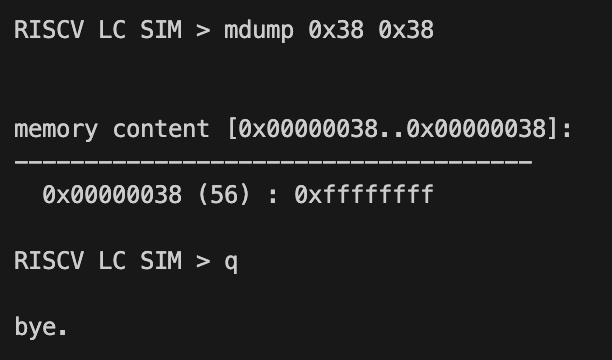
\includegraphics[width=1\linewidth]{../figs/add4-after-1.png}
    \end{figure}
    
    \begin{figure}[H]
        \caption{count10 result}
        \centering
        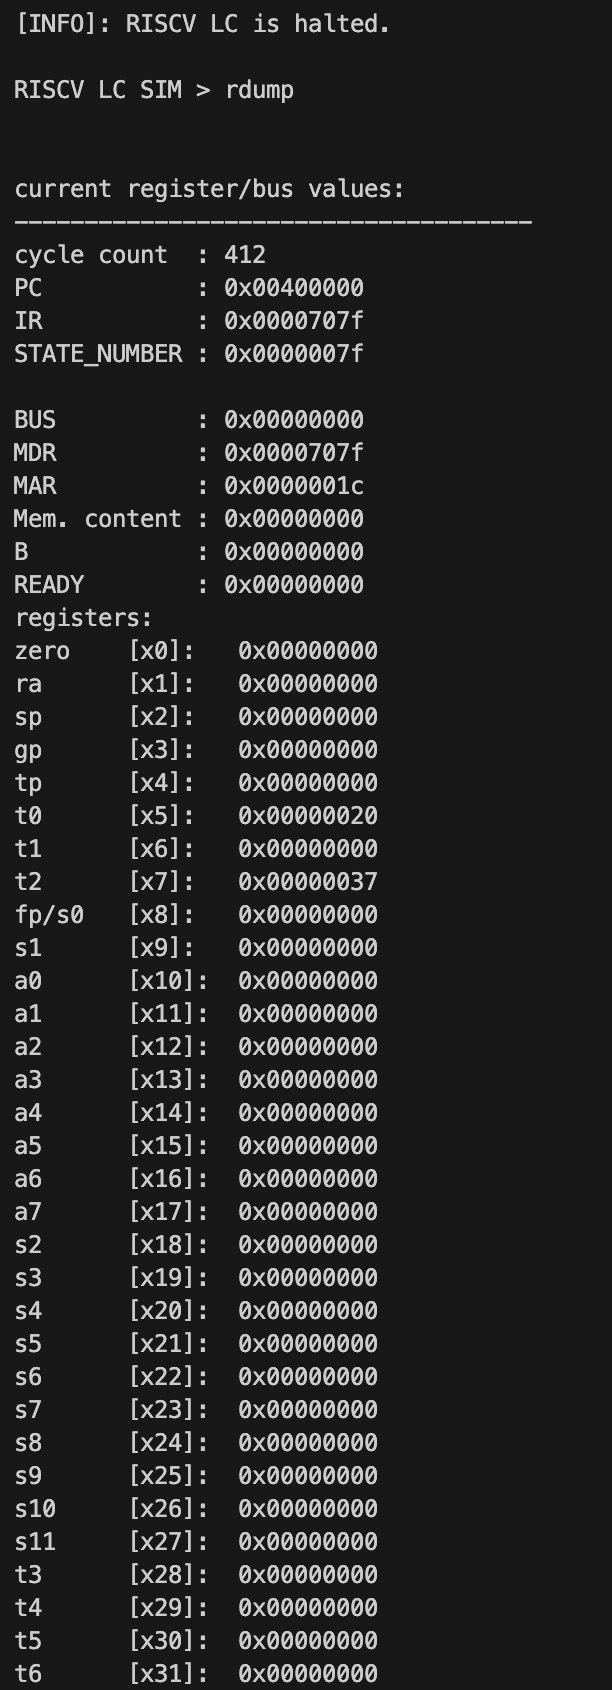
\includegraphics[scale=0.8]{../figs/count10-1.png}
    \end{figure}
    
    \begin{figure}[H]
        \caption{isa register values}
        \centering
        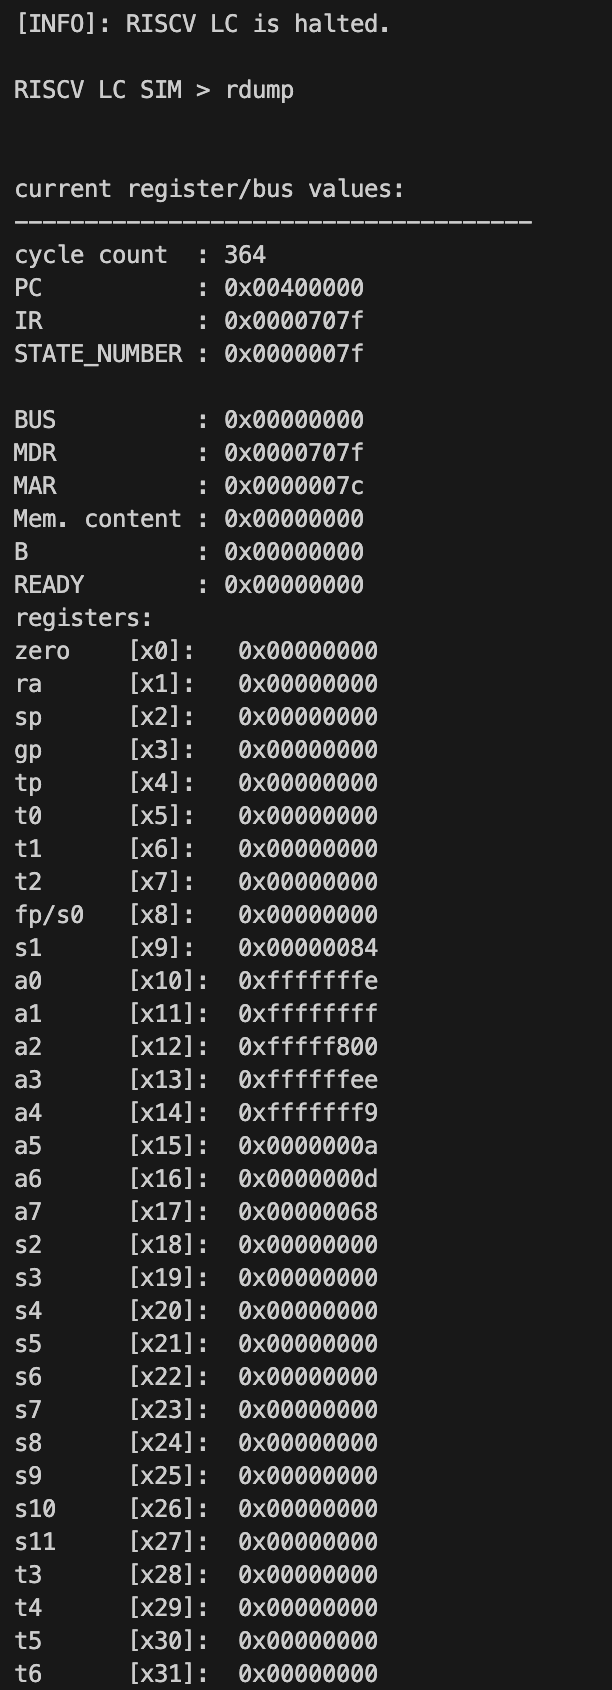
\includegraphics[scale=0.5]{../figs/isa-rdump.png}
    \end{figure}
    \begin{figure}[H]
        \caption{isa memory content}
        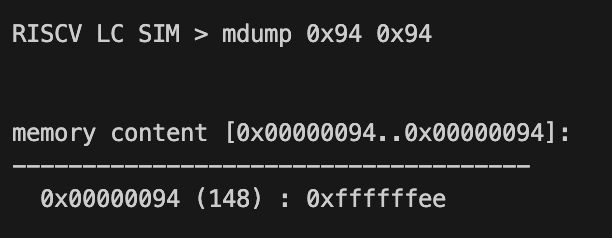
\includegraphics[width=1\linewidth]{../figs/isa-mdump.png}
    \end{figure}
    
    \begin{figure}[H]
        \caption{swap before}
        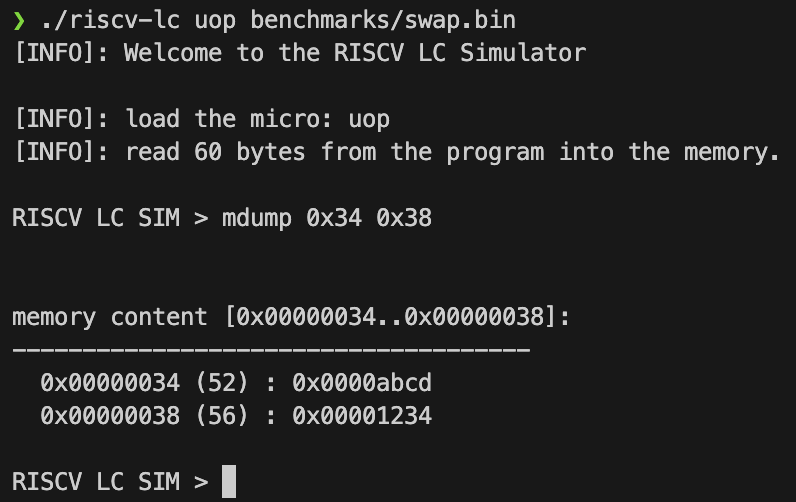
\includegraphics[width=1\linewidth]{../figs/swap-before-1.png}
    \end{figure}
    \begin{figure}[H]
        \caption{swap after}
        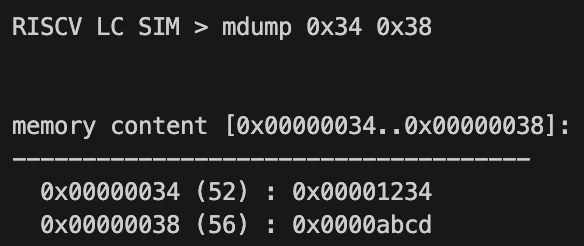
\includegraphics[width=1\linewidth]{../figs/swap-after-1.png}
    \end{figure}
\end{ans}
\pagebreak

\begin{qNoMark}
Lab 3.3 result
\end{qNoMark}

\begin{ans}
    \begin{figure}[H]
        \caption{add4 before}
        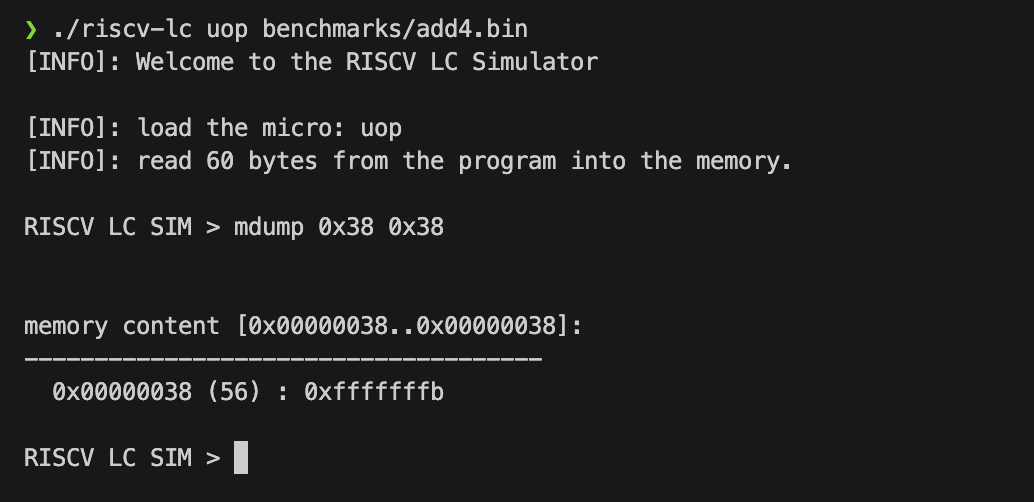
\includegraphics[width=1\linewidth]{../figs/add4-before-1.png}
    \end{figure}
    \begin{figure}[H]
        \caption{add4 after}
        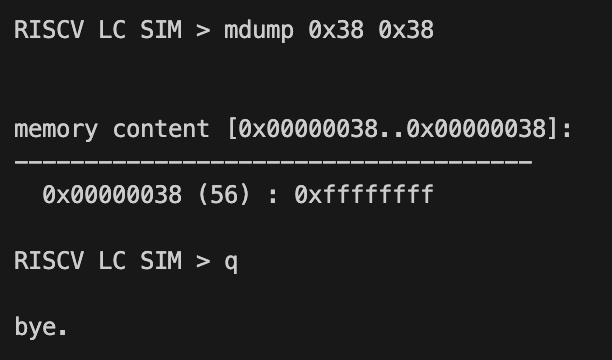
\includegraphics[width=1\linewidth]{../figs/add4-after-1.png}
    \end{figure}
    
    \begin{figure}[H]
        \caption{count10 result}
        \centering
        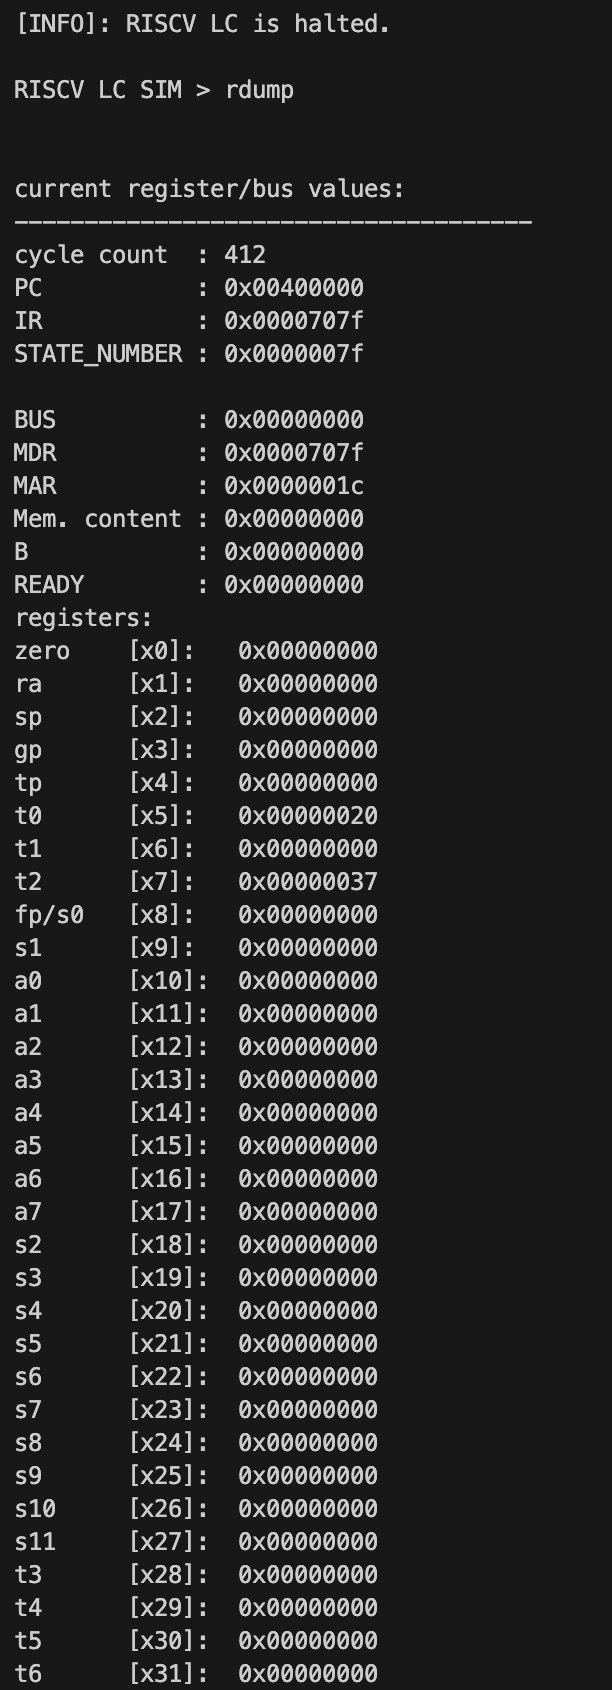
\includegraphics[scale=0.8]{../figs/count10-1.png}
    \end{figure}
    
    \begin{figure}[H]
        \caption{isa register values}
        \centering
        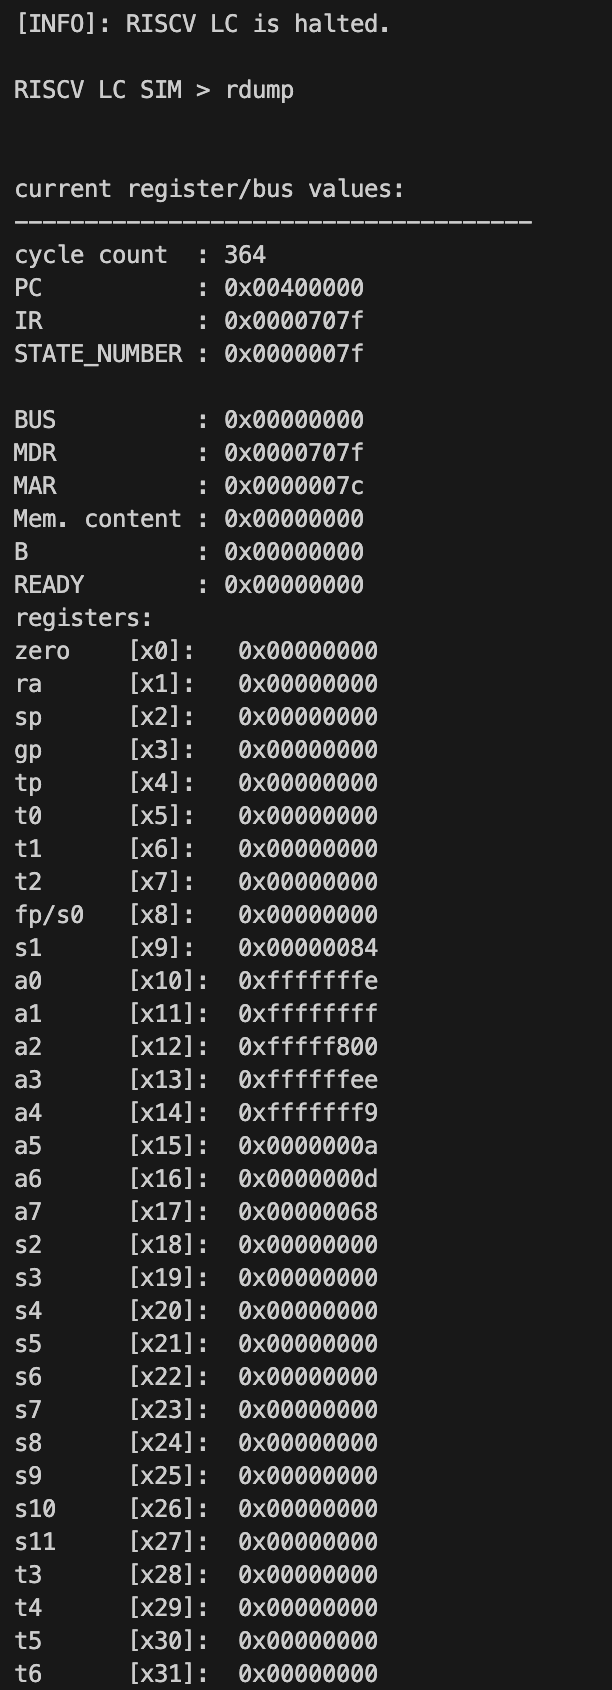
\includegraphics[scale=0.5]{../figs/isa-rdump.png}
    \end{figure}
    \begin{figure}[H]
        \caption{isa memory content}
        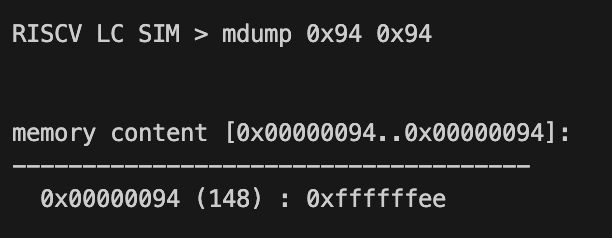
\includegraphics[width=1\linewidth]{../figs/isa-mdump.png}
    \end{figure}
    
    \begin{figure}[H]
        \caption{swap before}
        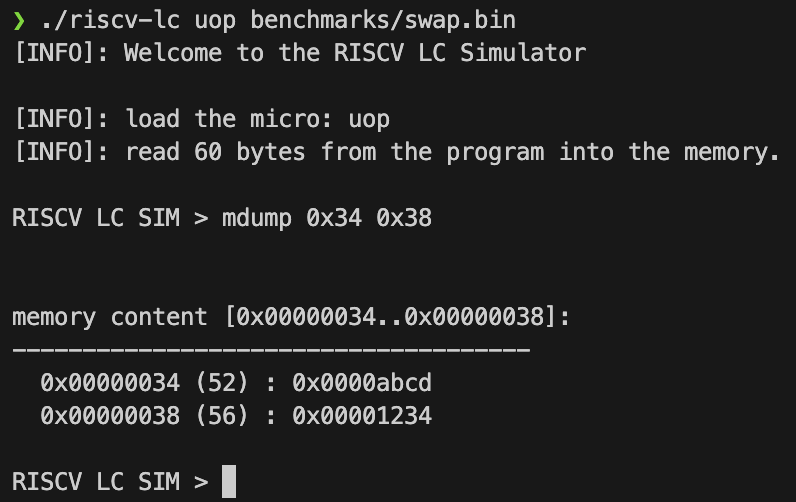
\includegraphics[width=1\linewidth]{../figs/swap-before-1.png}
    \end{figure}
    \begin{figure}[H]
        \caption{swap after}
        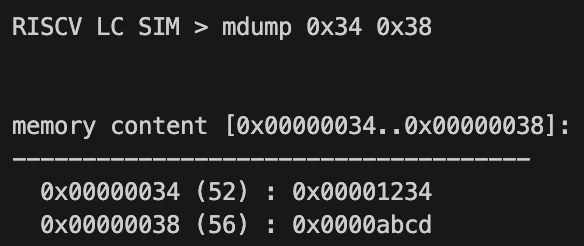
\includegraphics[width=1\linewidth]{../figs/swap-after-1.png}
    \end{figure}
\end{ans}

\end{document}
